\section{TCP/NC的实现}
%%数据包编码
\subsection{数据包编码}
%%有限域
\begin{frame}[t]
	\frametitle{有限域}
	\vspace{-1em}
	\begin{block}{有限域}
		有限域提供了一个有限集,
		在该有限集上明确定义且有效地实现了加法、减法、乘法和除法运算,
		并允许系统使用矩阵、行列式、高斯消元等线性代数中常见的运算工具来解决该域上的联立线性方程组问题。
	\end{block}
	\begin{columns}
		%%第一列
		\begin{column}{0.5\textwidth}
			\begin{table}[htp]
				\centering
				\label{tab:youxianyujia}
				\begin{tabular}{l|llll}
					\toprule
					+&0&1&A&B\cr
					\midrule
					0&0&1&A&B\cr
					1&1&0&A&B\cr
					A&A&B&0&1\cr
					B&B&A&1&0\cr
					\bottomrule
				\end{tabular}
			\end{table}
		\end{column}
		%%第二列
		\begin{column}{0.5\textwidth}
			\begin{table}[htp]
				\centering
				\label{tab:youxianyucheng}
				\begin{tabular}{l|llll}
					\toprule
					.&0&1&A&B\cr
					\midrule
					0&0&0&0&0\cr
					1&0&1&A&B\cr
					A&0&A&B&1\cr
					B&0&B&1&A\cr
					\bottomrule
				\end{tabular}
			\end{table}
		\end{column}
	\end{columns}
	\note{
		TCP/NC中需要对数据包进行编码,
		而从TCP层下到NC层的数据包都是字节流。
		如何抽象出前面谈到的报文概念?如何对数据包进行各种操作,如加减乘除?
		有限域为我门提供了一个数学工具。
	}
\end{frame}
%%编码示例
\begin{frame}
	\frametitle{编码示例}
	我们以两个数据包$p_{1}$和$p_{2}$的运算为例,
	说明如何对数据包进行编码。
	假定数据包$p_{1}$和$p_{2}$都为一个2字节的报文,
	以比特流的形式表示,
	$p_{1}=\{1010\ 0101\ 0110\ 1111\}$,$p_{2}=\{1111\ 0000\ 1101\ 0110\}$,
	我们需要计算$p_{encoded}=7p_{1} \oplus 13p_{2}$的值。
	步骤如下:
	\begin{enumerate}[(1)]
		\item 取$p_{1}$和$p_{2}$的第一个字节,
		分别是$\{1010\ 0101\}$和$\{1111\ 0000\}$,
		对应的十进制为$D_{p_1}=165$和$D_{p_2}=240$。
		在有限域$GF(2^8)$下计算$7\times 165$和$13 \times 240$的值,
		分别是$0xc6$和$0xc4$。
		则$p_{encoded}$的第一个字节为$0xc4 \oplus 0xc6=0x02$,
		二进制表示为$\{0000\ 0010\}$。
		\item 同样的方法处理$p_{1}$和$p_{2}$的第二个字节,
		结果为$\{1010\ 0111\}$。
		\item 拼接两个结果得到$p_{encoded}=\{0000\ 0010\ 1010\ 0111\}$。
	\end{enumerate}
\end{frame}
\subsection{技术路线}
%%设备选型
\begin{frame}
	\frametitle{设备选型}
	\begin{columns}
		\begin{column}{0.4\textwidth}
			考虑到无人机视频传输的应用场景,
			及TCP/NC需要参与到网络协议栈的流程中去,
			选用Raspberry Pi这款基于Linux的嵌入式设备,
			部署TCP/NC协议,如图\ref{fig:rasp}所示。

		\end{column}
		\begin{column}{0.5\textwidth}
			\begin{figure}
				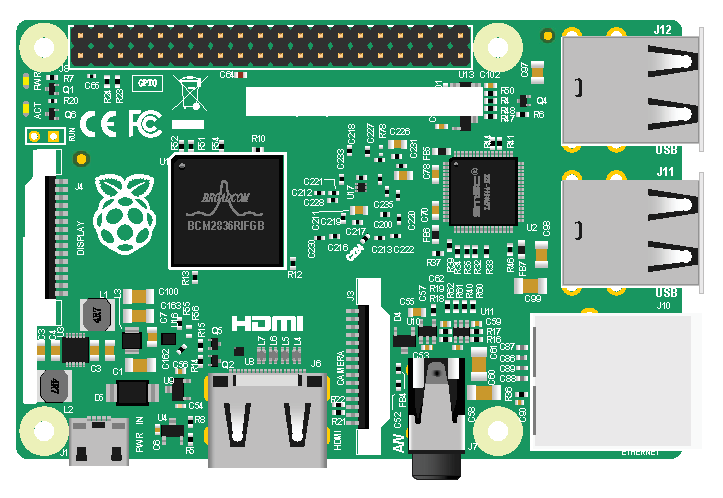
\includegraphics[height=4cm]{figures/rasp.eps}
				\caption{Raspberry Pi板子}
				\label{fig:rasp}
			\end{figure}
		\end{column}
	\end{columns}
	\note{
		Raspberry Pi是一款ARM架构的单板机,
		板载了以太网卡。支持CSI接口,
		方便外接摄像头,进行后期无人机视频传输测试。
		操作系统选择树莓派基金会的Debian系统,
		内核版本为3.18。
	}
\end{frame}
%%Netfilter
\begin{frame}
	\frametitle{Netfilter}
	\begin{columns}
		\begin{column}{0.5\textwidth}
			NC层实施方案有两种:
			\begin{enumerate}
				\item 直接在内核的TCP协议源码上更改,添加NC层的各个模块,然后再编译内核源码
				\item 利用Linux内核提供给用户用于处理网络封包的框架——Netfilter。
			\end{enumerate}
			本文将TCP/NC部署在Netfilter的NF\_IP\_LOCAL\_IN和NF\_IP\_LOCAL\_OUT处。
		\end{column}
		\begin{column}{0.4\textwidth}
			\vspace{-1.5em}
			\begin{figure}
				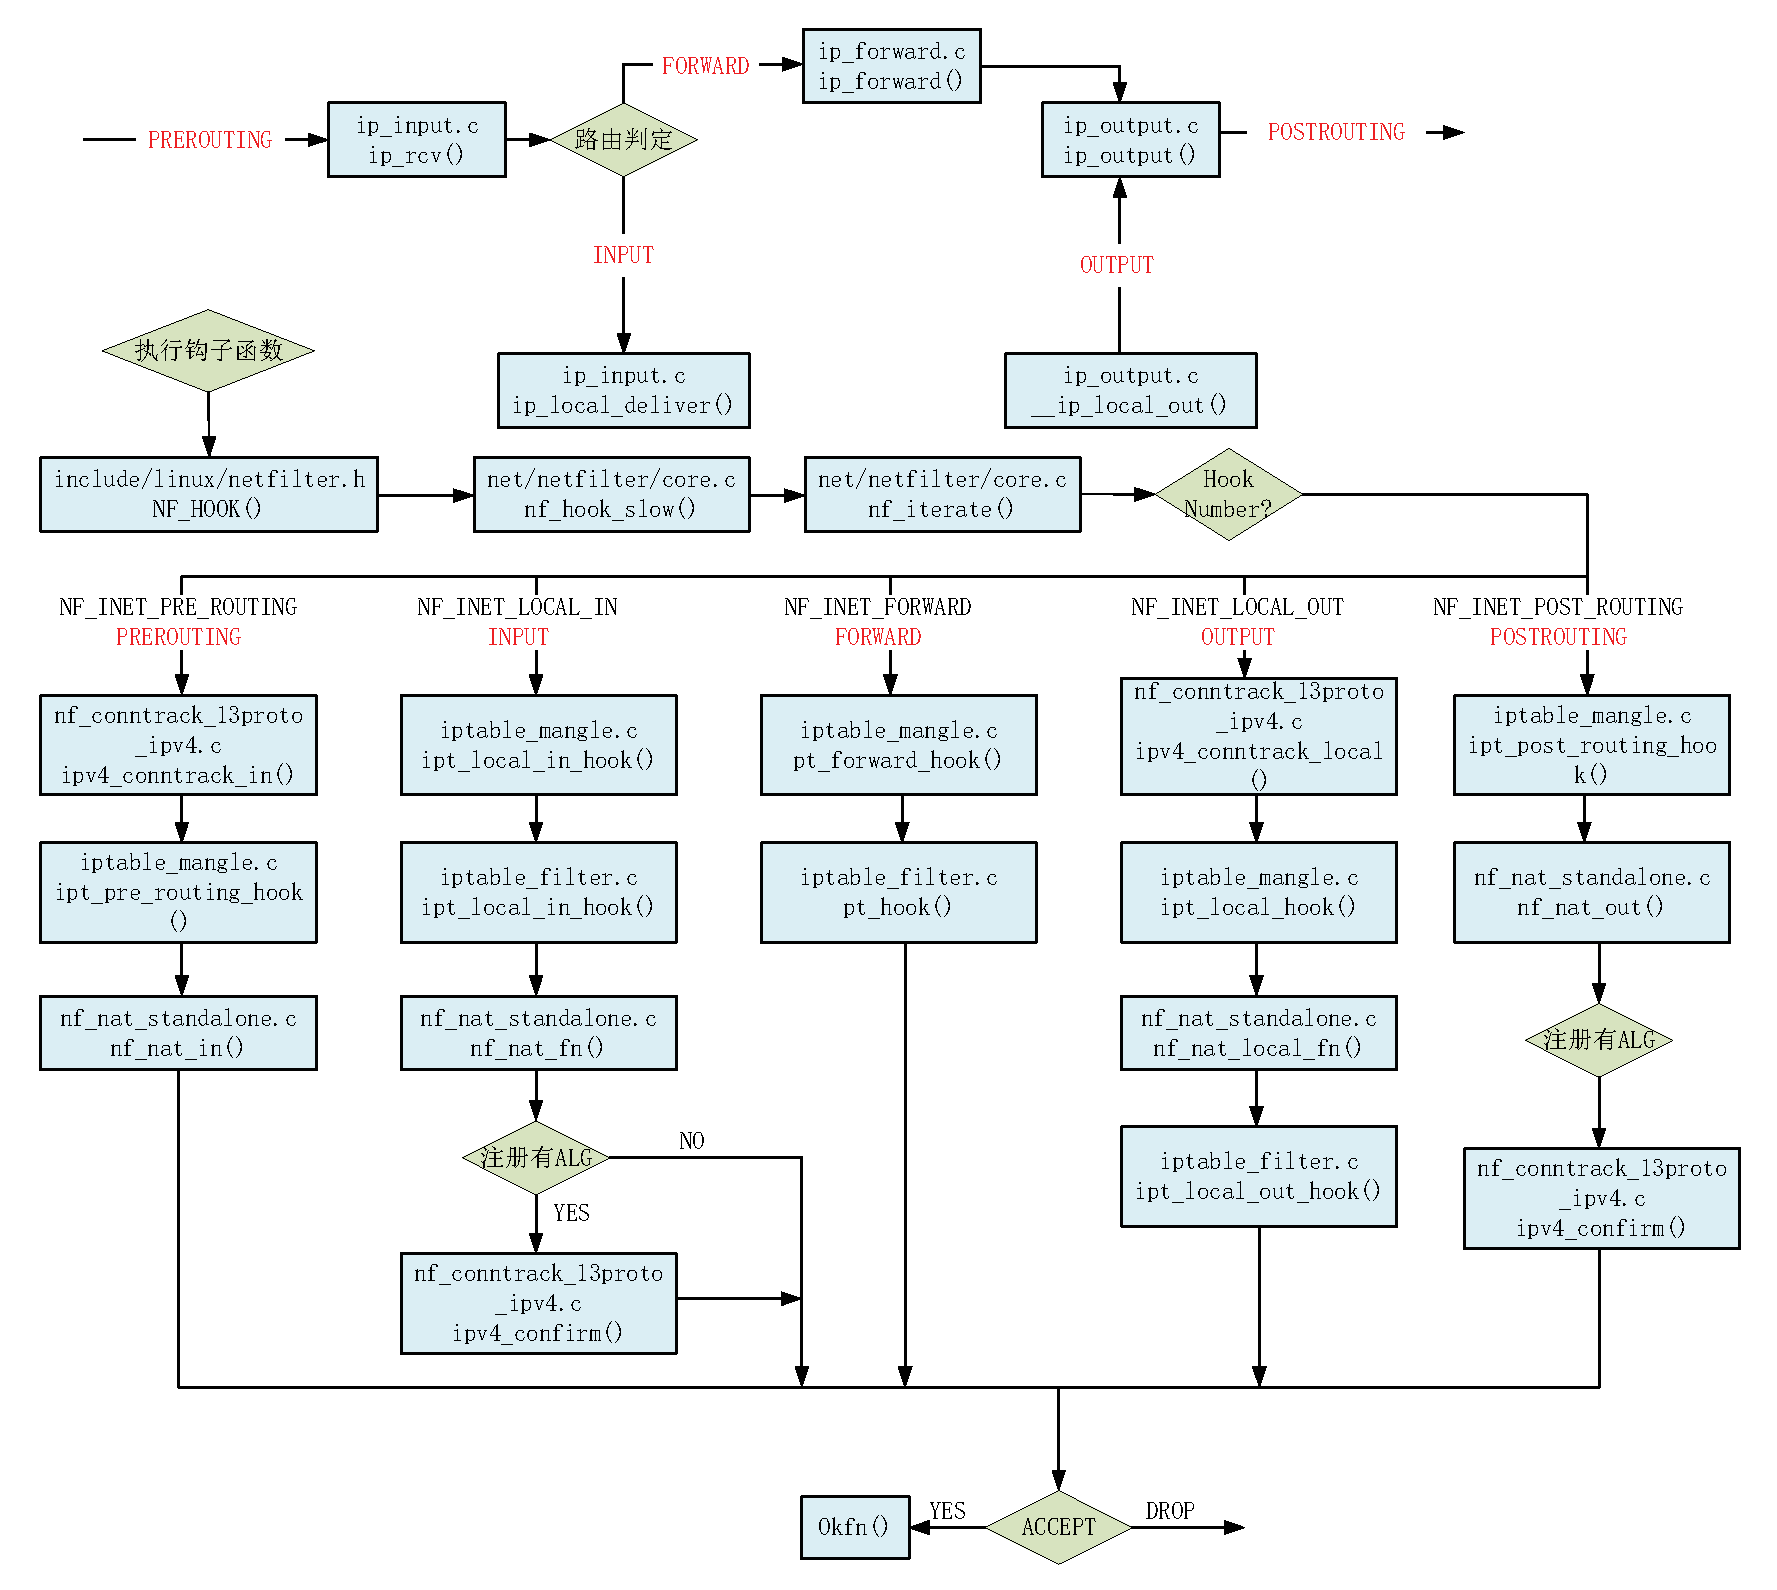
\includegraphics[height=5cm]{../figures/packetflow.eps}
				\caption{Netfilter及其在内核源码中调用关系}
				\label{fig:packetflow}
			\end{figure}
		\end{column}
	\end{columns}

	\note{
	}
\end{frame}
%%关键数据结构
\begin{frame}
	\frametitle{关键数据结构}
	NC层在NF\_IP\_LOCAL\_IN和NF\_IP\_LOCAL\_OUT这两个钩子点获得的都是单独的报文,
	其形式为\emph{sk\_buff}结构体,如图\ref{fig:skbuff}所示。
		\begin{columns}
		\begin{column}{0.5\textwidth}
			数据包在Linux的网络协议栈的不同层之间传递,
			其体现形式就是不同层的函数对一个数据包对应的\emph{sk\_buff}进行各种操作。
			\\
			TCP/NC通过\emph{sk\_buff}获得数据包的字节流,
			然后对数据包进行编码。
		\end{column}
		\begin{column}{0.4\textwidth}
			\vspace{-1.5em}
			\begin{figure}
				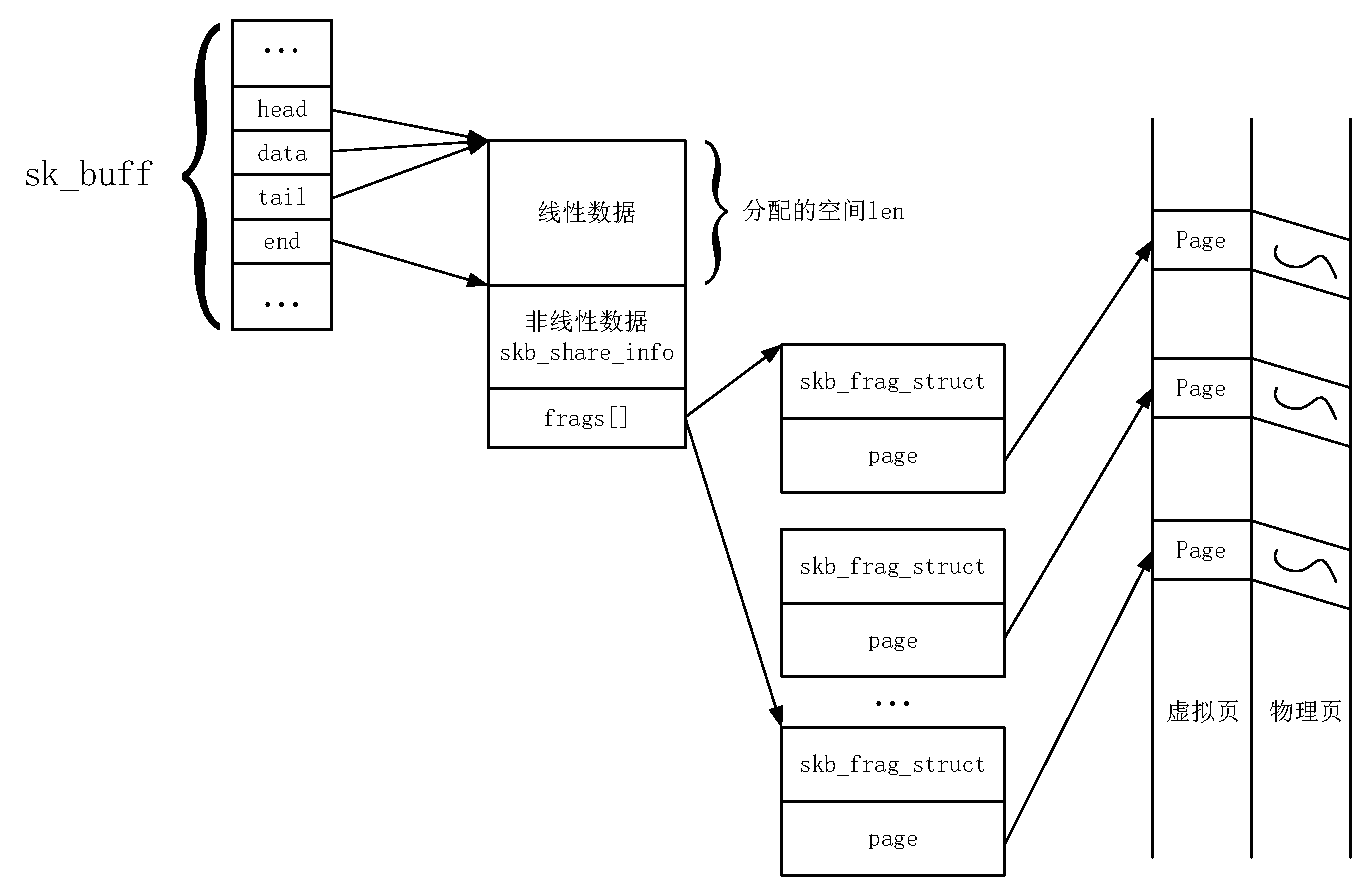
\includegraphics[height=4cm]{../figures/skbuff.eps}
				\caption{skbuff结构}
				\label{fig:skbuff}
			\end{figure}
		\end{column}
	\end{columns}
	
\end{frame}
\subsection{NC层关键技术}
%%NC层头部
\begin{frame}
	\frametitle{NC层头部}
	\begin{columns}
		\begin{column}{0.4\textwidth}
			发送端需要给编码得到的编码包添加NC头部,
			包括编码系数等信息,接收端利用这些信息进行解码。
			图\ref{fig:codingMechanism}为NC报文的头部。
		\end{column}
		\begin{column}{0.6\textwidth}
			\begin{figure}
				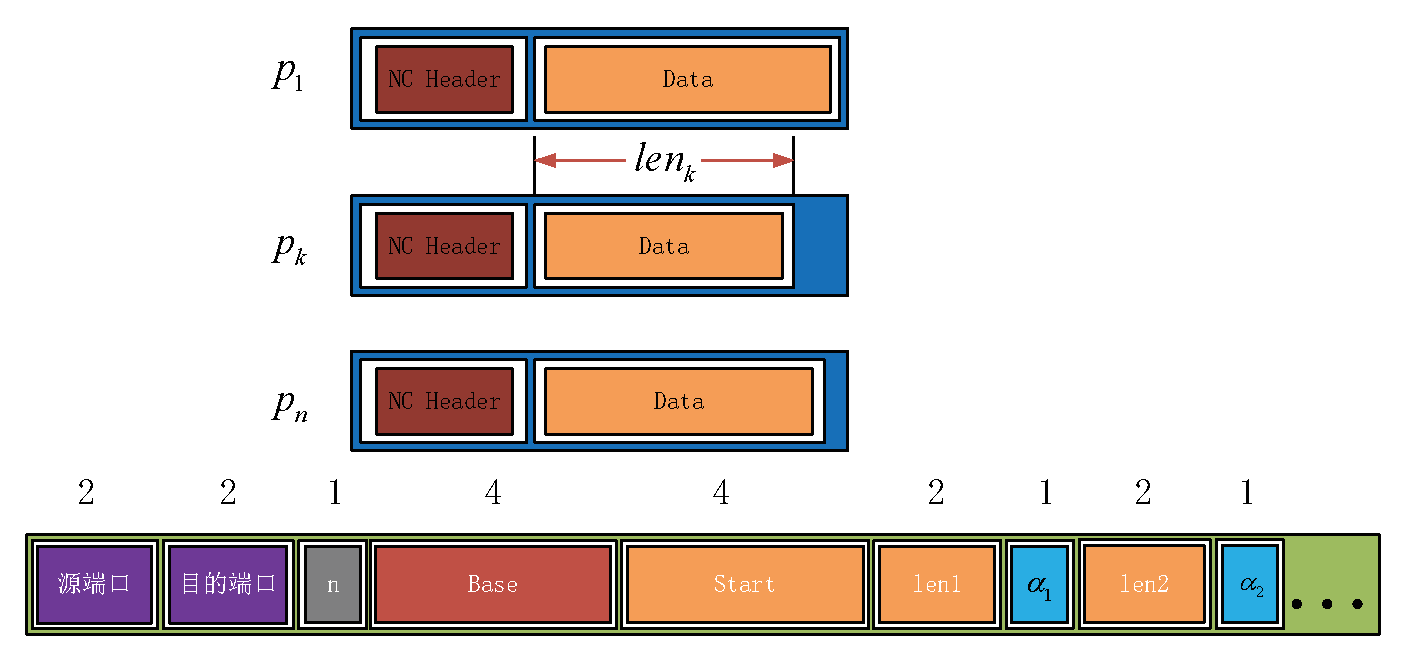
\includegraphics[height=4cm]{../figures/codingheader.eps}
				\label{fig:codingheader}
				\caption{NC层头部}
			\end{figure}
		\end{column}
	\end{columns}
\end{frame}
%%编码端
\begin{frame}
	\frametitle{编码步骤}
	\renewcommand{\algorithmcfname}{算法}
	\begin{algorithm}
		\caption{对数据包进行编码} 
		\label{algo:bianma}
		\SetKwInOut{Input}{\textbf{输入}}\SetKwInOut{Output}{\textbf{输出}}
		\Input{\\
			冗余度因子 $R$;\\
			编码缓存双向链表 $sk\_buff\_head$;\\
			冗余度残留系数 $NUM$;\\
			编码窗口 $TCPNC\_CODE\_WND$;
		}
		\Output{\\
			编码报文链表 $sk\_buff\_ret$
		}
		$NUM \leftarrow NUM+R$;\\
		\While{$NUM \ge 1$}  
		{  
			从$sk\_buff\_head$表头开始往后遍历$TCPNC\_CODE\_WND$个报文;\\
			在$GF\left(2^8\right)$上生成$TCPNC\_CODE\_WND$个系数;\\
			根据系数和原始数据包计算出编码包;\\
			给编码报文添加NC头部;\\
			将编码包加入到$sk\_buff\_ret$链表;\\
			$NUM \leftarrow NUM-1$;
		}
		\Return \ $sk\_buff\_ret$;
	\end{algorithm}
\end{frame}

%\subsection{解码矩阵}
\frame{
	\frametitle{解码矩阵}
\begin{columns}[onlytextwidth]
	%%\vspace{5em}
	\hspace{-2.0em}
	\begin{column}{0.55\textwidth}
		%%\vspace{-4em}
		\begin{figure}
			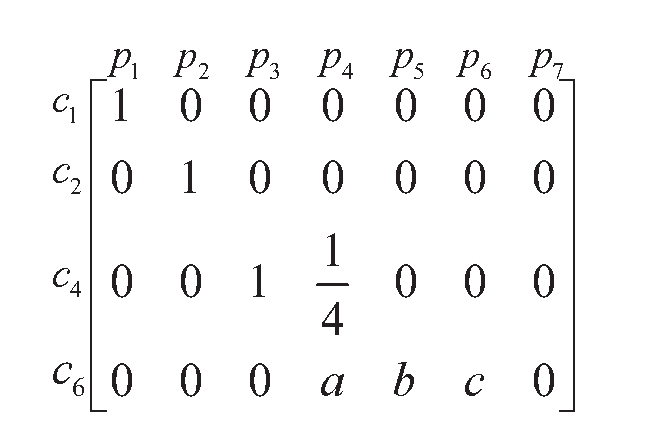
\includegraphics[height=3cm]{figures/matrix.eps}
			\caption{解码矩阵示例}
			\label{fig:jiema}
		\end{figure}
	\end{column}
	\hspace{0.5em}
	\begin{column}{0.55\textwidth}
		\footnotesize
		\begin{block}{解码矩阵}
		图\ref{fig:jiema}表示接收端的解码矩阵的一个示例。
		编码报文$c_3$丢失,$c_4$正确收到,$c_5$又丢失。
		可以看到,接收端可以解码出$p_1$和$p_2$,
		看到(see)$p_3$和$p_4$,
		无法解出$p_3 \sim p_6$。
		\end{block}
%	\begin{block}{信息}
%		
%		\end{block}
	\end{column}
\end{columns}
%\vspace{2em}
以图\ref{fig:jiema}为例,
解码矩阵还需要2个由$p_3$到$p_6$组成的编码包即可解码出$p_3$和$p_6$。
如果能让发送端了解到这个信息,
发送端在下一回合发送过程中,
主动额外地多发相关的编码包,
就可以提前解出$p_3 \sim p_6$,
而无需等到下一次根据冗余度发出的冗余包。
}
%\subsection{NC头部设计}
\frame{
	\frametitle{NC头部结构}
	\vspace{-2em}
	\begin{figure}
	\hspace{-1.5em}
		%\centering
		%%\hspace{-em}
		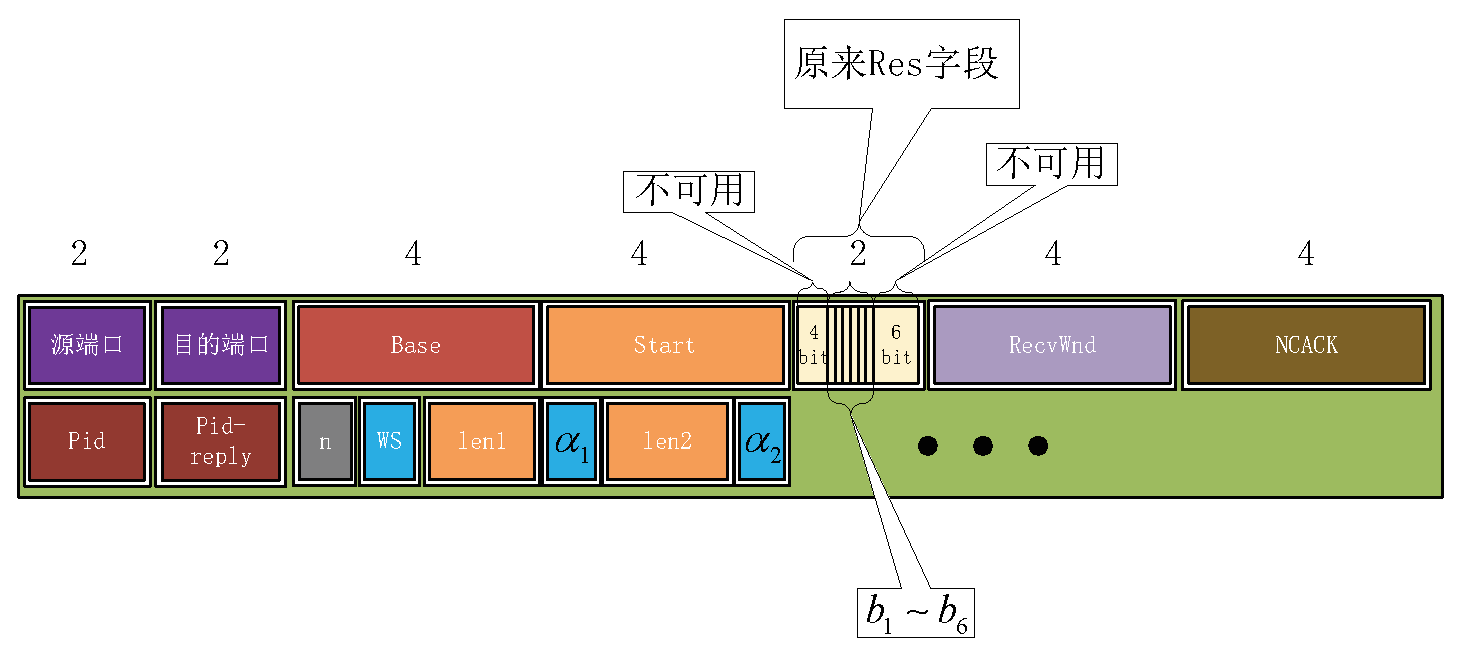
\includegraphics[height=2.8cm]{figures/newheader.eps}
		\caption{新NC头部设计}
		\label{fig:ncheader}
	\end{figure}
图\ref{fig:ncheader}展示的NC头部中添加了\emph{Pid}和\emph{Pid-reply}两个字段。
\emph{Pid}表示编码报文的编号;
如果此报文为ACK报文的话,
\emph{Pid-reply}表示这个ACK报文是由编号为\emph{Pid-reply}的报文激发的。
}
%\subsection{反馈重传流程设计}
\frame{
	\frametitle{获码矩阵信息}
	\begin{block}{发送端}
		对于发出去的每个编码包,
		若其编号为\emph{Pid},
		记录编号为\emph{Pid}的编码包由哪几个原始数据包组成,
		以图\ref{fig:codingexp}为例,
		\emph{Pid=1}的编码包由$p_1$、$p_2$、$p_3$和$p_4$组成。
		\\
	\end{block}
	\begin{block}{接收端}
		接收端在发出去的每个ACK报文中都会填写NC头部的\emph{Pid-reply}字段,
		表示此ACK报文是由发送端的编号为\emph{Pid-reply}的编码报文激发的。
	\end{block}
}
%\frame[allowframebreaks]{
\begin{frame}
	\frametitle{获取接收端解码矩阵信息}
	%\vspace{-2em}
	\begin{myDef}[矩阵可解状态]\label{def:kejie}
		假定接收端收到的序号最大的报文为$p_j$,
		已经确认的序号最大的报文为$p_i$。
		如果$i=j$,那么就说接收端解码矩阵为可解状态。
	\end{myDef}
发送端的处理过程如下:
	\begin{block}{步骤}
		%\footnotesize
		\begin{enumerate}[<+-|alert@+>]
			\item 提取\emph{Pid-reply}域,
			罗列值为\emph{Pid-reply}的编码包的所有原始数据包$p_i \sim p_j(i \le j)$;
			\item 如果ACK报文的确认序号$ACK=p_k$,
			那么可知接收端解码矩阵在收到编号为\emph{Pid=Pid-reply}的编码报文时,
			缺失$j-k+1$个编码包才可以变为可解状态;
			%\framebreak

		\end{enumerate}
	\end{block}
%}
\end{frame}


\begin{frame}
		\frametitle{获取接收端解码矩阵信息}
		\begin{block}{步骤( 接上页)}
		\begin{enumerate}[<+-|alert@+>]
	\addtocounter{enumi}{2}
				\item 更新\emph{loss}和\emph{last\_loss}变量,
	其中\emph{loss}表示接收端解码矩阵变为可解状态所需的组合包个数,\emph{last\_loss}表示\emph{loss}上一次的值。
	\item  计算当前时间$T_{now}$和上一次补偿重传的时间$T_{last}$的差值是否超过RTO。
	如果超过,那么重传当前编码缓存窗口的前\emph{loss}个报文;
	如果未超过,比较\emph{loss}的\emph{last\_loss}的值,
	如果$loss \le last\_loss$,那么不进行补偿重传,
	如果$loss > last\_loss$,说明在$T_{last}$到$T_{now}$这段时间又有报文丢失,
	那么就重传编码缓存窗口的前$loss-last\_loss$个报文。
		\end{enumerate}
		\end{block}
\end{frame}

\begin{frame}
	\frametitle{流程图}
	\begin{figure}
		\hspace{-1.5em}
		%\centering
		%%\hspace{-em}
		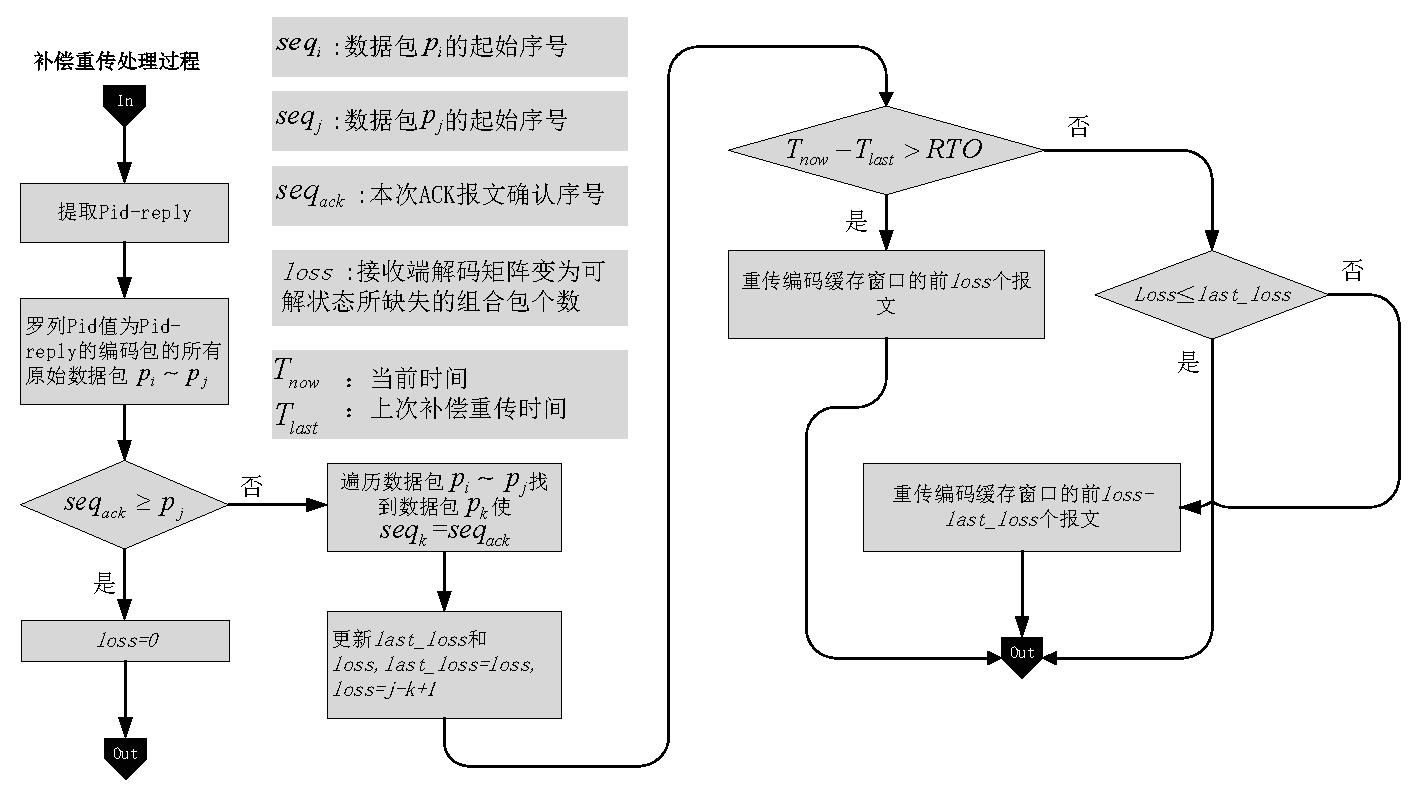
\includegraphics[height=5cm]{../figures/bccc.eps}
		\caption{补偿重传流程图}
		\label{fig:buchang}
	\end{figure}
\end{frame}

\section{E-TCP/NC}